\documentclass{beamer}
\usetheme{Stats}
\setbeamercovered{transparent}
\usepackage{color}
\usepackage{hyperref}
  \hypersetup{
      colorlinks=true
        linkcolor=black
        }
\usepackage{url}
\usepackage{graphics}
\usepackage{tikz}
\usepackage{booktabs}


%%%%%%%%%%%%%%%%%%%%%%%%%%%%%%%% Title Slide %%%%%%%%%%%%%%%%%%%%%%%%%%
\title[]{Measuring International Financial Supervisory Transparency}
\author[]{
    \href{mailto:gandrud@hertie-school.org}{Christopher Gandrud}, Mark Copelovitch, and Mark Hallerberg
}
\date{\today}

\begin{document}

\frame{\titlepage}

\section{Motivation}
    \frame{
        \frametitle{Why financial supervisory transparency?}
        Financial supervisory transparency has been \textbf{lauded} as promoting:

        \begin{itemize}
                \item financial system stability,
        \item democratic legitimacy for supervisors.
        \end{itemize}

    }

    \frame{
        \frametitle{Promotion}
            Supervisory transparency has been \textbf{promoted} by international/supra-national institutions including the IMF, Basel Committee, and the European Union for these reasons.
    }

    \frame{
        \frametitle{But\ldots}

    We \textbf{{\large{lack}} reliable}, \textbf{cross-country}, and \textbf{cross-time} indicators of financial supervisory transparency to \textbf{{\large{test}}} these assertions.
    }

    \frame{
        \frametitle{Objective}
        Our objectives are to:
        \begin{itemize}
            \item \textbf{Develop} a reliable and valid indicator of supervisory transparency across countries and time.
                \begin{itemize}
                    \item Largely complete.
                \end{itemize}
            \item Use this to \textbf{examine}:
                \begin{itemize}
                    \item \textbf{why} countries become more/less transparent,
                    \item \textbf{how}, if at all supervisory transparency affects economic outcomes.
                \end{itemize}
        \end{itemize}
    }

    \frame{
        \frametitle{Methodological Contribution}
        Our indicator makes (at least) two important methodological contributions:
        \begin{itemize}
            \item Develop a Hierarchical Bayesian Item Response Theory-based \textbf{unique indicator} of countries' \textbf{willingness to credibly} reveal basic facts about their \textbf{financial systems to international actors}.
            \item Show that \textbf{missing financial system data} is \textbf{often endogenous} to financial system difficulties and policymaker's aspirations.
        \end{itemize}
    }

    \section{Creating the FRT Index}
    \frame{
        \frametitle{Predecessors}
        Recent supervisory transparency indexes generally use \textbf{surveys} and then \textbf{sum} dichotomous responses.
        \begin{itemize}
            \item<1-> Lierdorp et al. (2013)
            \item<1-> Arnone, Darbar, and Gambini (2007) (based on classified IMF data set, data is not publicly available)
            \item<1-> Seelig and Novoa (2009)
            \item<1-> Masciandaro, Quintyn, and Taylor (2008)
        \end{itemize}
    }

    \frame{
        \frametitle{Issues with previous methods}
        There are a number of issues with previous methods:
        \begin{itemize}
        	   \item Ironically, many of the surveys are \textbf{not transparent}.
            \item Survey methods are \textbf{laborious}.
            \item Surveys rely on \textbf{temporally ephemeral} information.
            \item So, survey methods provide only brief windows, \textbf{not time series}.
            \item Summing responses \textbf{assumes} that each item should be \textbf{weighted equally}.
            \item \textbf{High non-response rate} (Liedorp et al. had a response rate of 57\%). This information is often \textbf{ignored}.
            \item \textbf{No estimation of uncertainty}.
        \end{itemize}
    }

    \frame{
        \frametitle{Our Approach}
        We build on \textbf{Hollyer et al.‘s (2014)} approach to constructing a transparency indicator (also Stan Development Team (2014)). \\[0.5cm]

    Treat financial regulatory transparency (FRT) as an \textbf{unobserved latent variable}.\\[0.5cm]

     Our \textbf{FRT Index} summarizes countries'�� \textbf{likelihood of reporting} yearly data to indices included in the World Bank's Global Financial Development Database (\textbf{GFDD}).
    }

    \frame{
        \frametitle{Observations and items}
        60 \textbf{high income countries}, 22 years (\textbf{1990-2011}), 14 \textbf{items}.
    }

    \frame{
        \frametitle{The model}
        $$
            y_{k,c,t} = \left\{ \begin{array}{ll}
                            1 & \mathrm{if\; item}\; k\; \mathrm{reported\; in\; country}\; c,\; \mathrm{year}\; t \\
                            0 & \mathrm{if\; item}\; k\; \mathrm{not\; reported\; in\; country}\; c,\; \mathrm{year}\; t
            \end{array} \right.
        $$

        Esimate (from Stan Development Team (2014, 49-50)):

        $$
            \mathrm{Pr}(y_{k,c,t} = 1 |\alpha_{c,t}) = \mathrm{logit}[\exp(\log\gamma_{k})*(\alpha_{c,t} - \beta_{k} + \delta)]
        $$

        where:

        \begin{itemize}
            \item $\alpha_{c,t}$ is the estimated propensity for country $c$ at year $t$ to report item $k$. This can be thought of as the \textbf{transparency} score.
            \item $\log\gamma_{k}$ is the \textbf{discrimination} parameter for item $k$
            \item $\beta_{k}$ is the \textbf{difficulty} parameter for item $k$
            \item $\delta$ is the \textbf{mean transparency}
        \end{itemize}
    }

    \frame{
        \frametitle{Priors (1)}
        $$
        \alpha_{c,1990} \sim \mathrm{N}(0,\;1)
        $$

        \begin{center}
            then rescentered by $\frac{\alpha_{c,1990}-\bar{\alpha_{1990}}}{SD_{\alpha,1990}}$
        \end{center}

        Then random-walk priors
        $$
            \alpha_{c,t} \sim N(\alpha_{c,t-1},\: \sigma_{\alpha c}) \forall t > 1
        $$

        where

        $$
            \sigma_{\alpha c} \sim Cauchy(0,\;0.25)
        $$
    }

    \frame{
        \frametitle{Priors (2)}
        \begin{equation}
            \begin{array}{lcl}
                \delta & \sim & Cauchy(0,\;0.25) \\

                \beta & \sim & N(0,\; \sigma_{\beta}) \\

                \log\gamma & \sim & N(0,\; \sigma_{\gamma})
            \end{array}
        \end{equation}

        where
        \begin{equation}
            \begin{array}{lcl}
                \sigma_{\beta} & \sim & Cauchy(0,\;0.25) \\

                \sigma_{\gamma} & \sim & Cauchy(0,\;0.25)
            \end{array}
        \end{equation}
    }

    \frame{
        \frametitle{Estimation}
        We estimated the model using \textbf{Stan}/No-U-Turn Sampler (good for highly correlated data).
    }


    \frame{
        \frametitle{What are we actually measuring?}
        The willingness of a country to report \textbf{minimally credible} information about its financial system \textbf{to international institutions and investors}.
    }

    \frame{
        \frametitle{FRT Index Overview (1990)}

        \begin{center}
            \includegraphics[scale=0.25]{figures/FRT_1990.pdf}
        \end{center}
    }

    \frame{
    \frametitle{FRT Index Overview (2011)}

    \begin{center}
        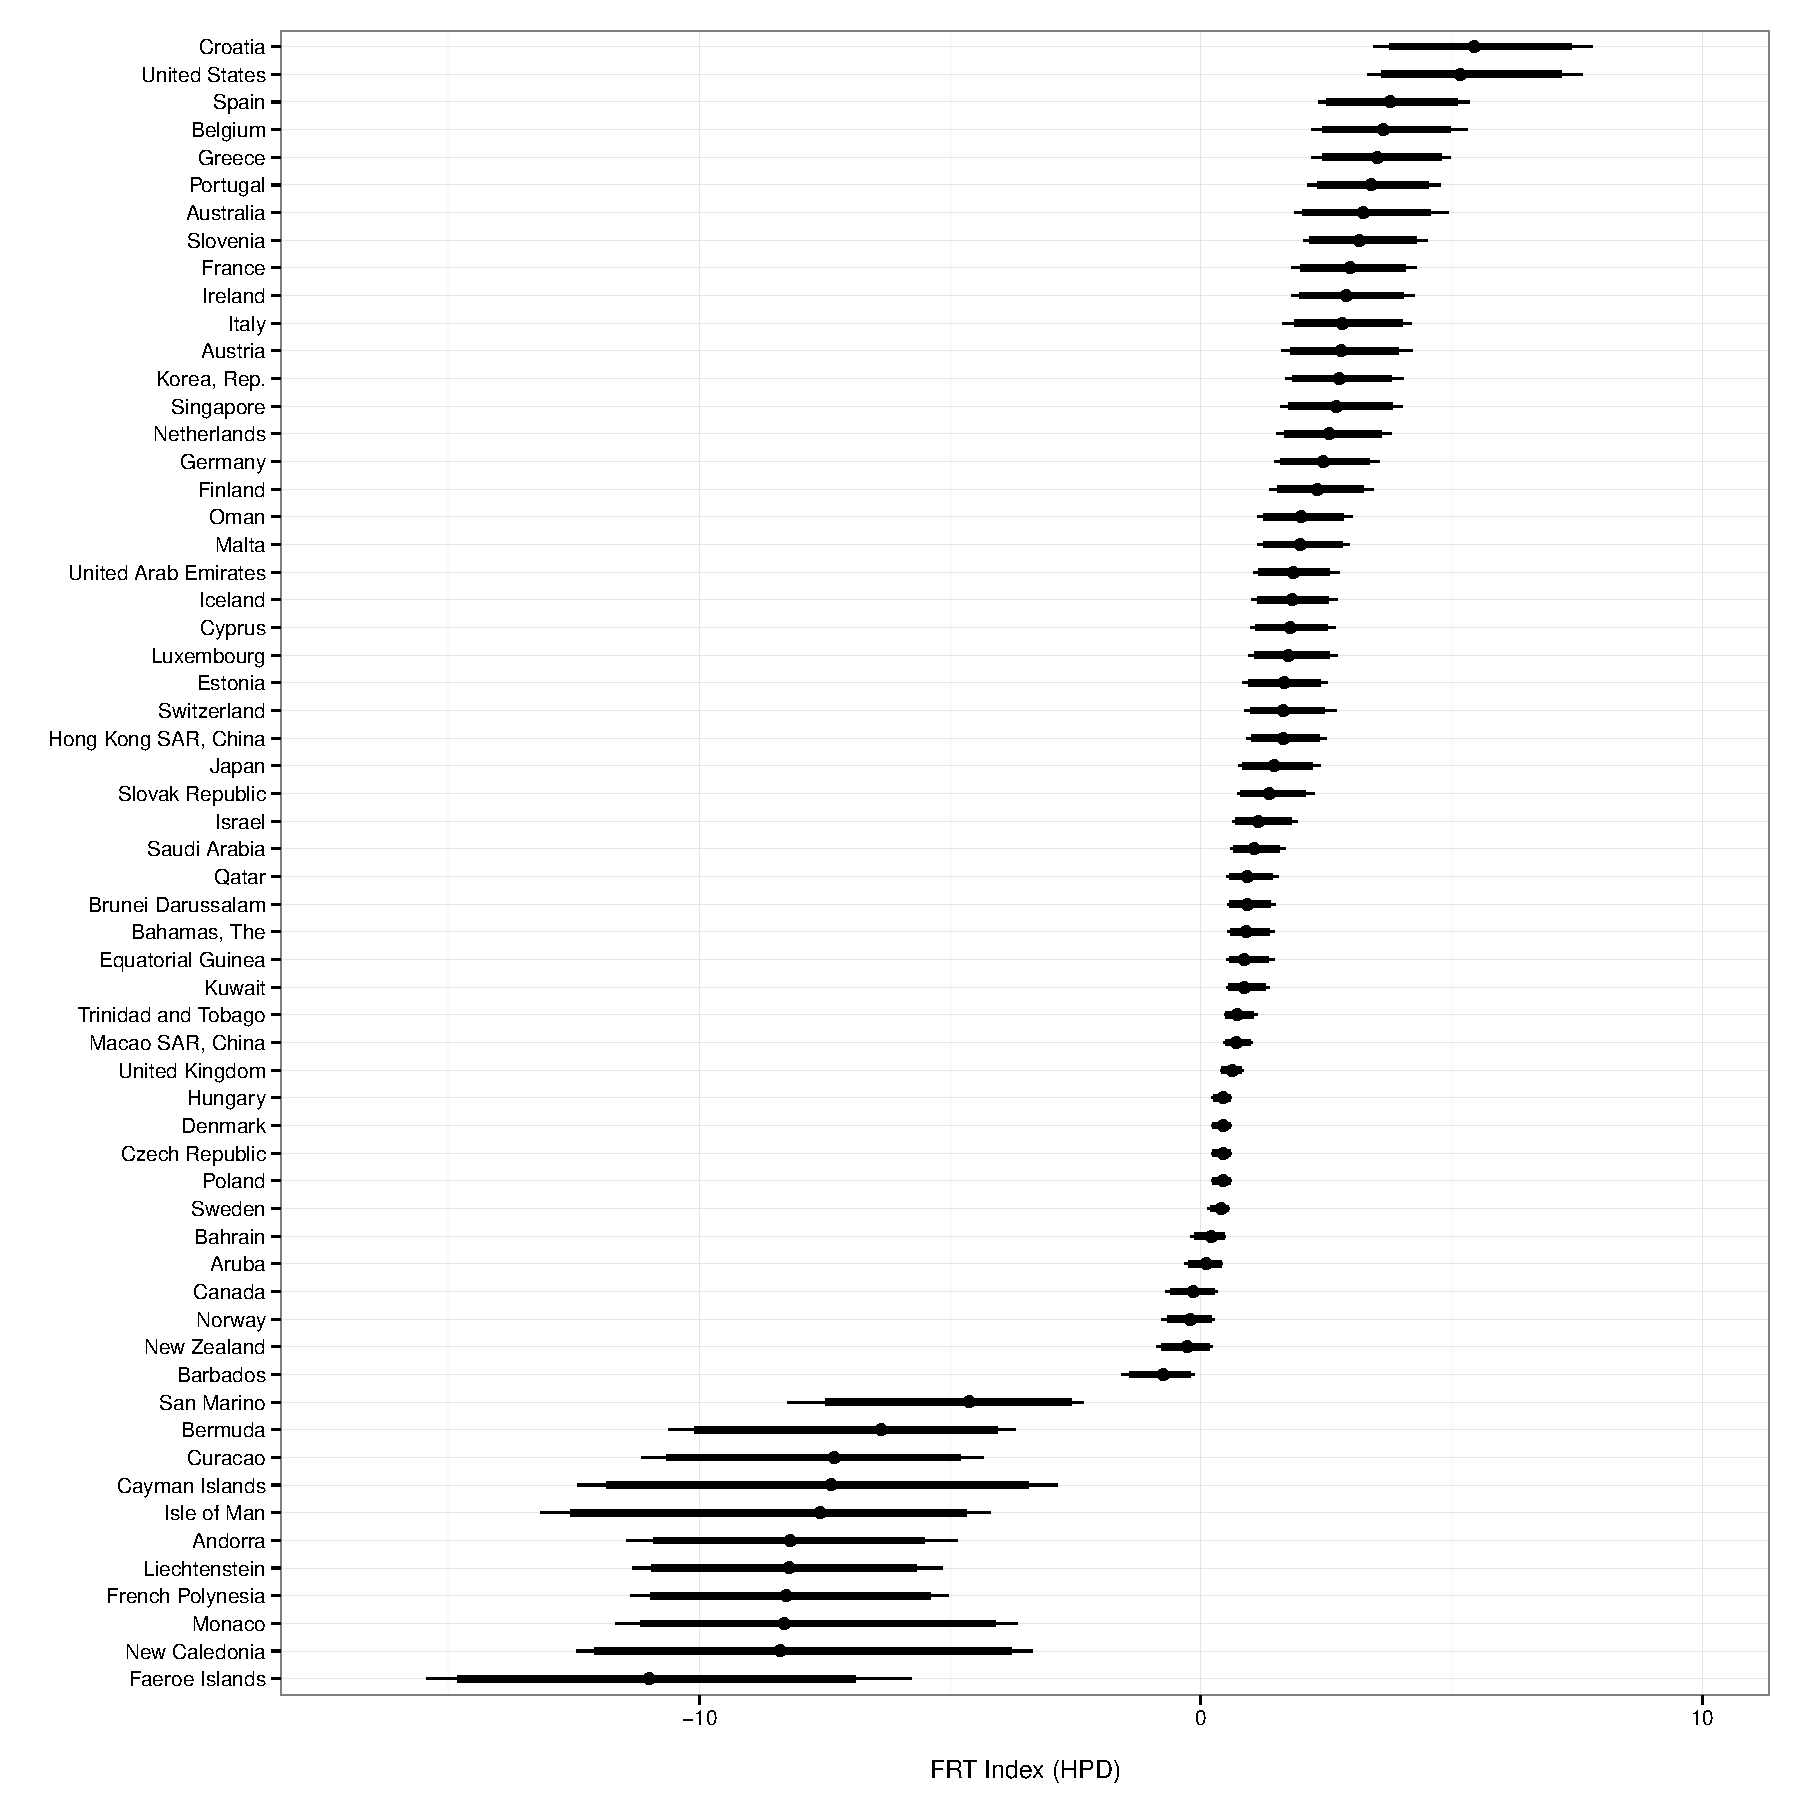
\includegraphics[scale=0.25]{figures/FRT_2011.pdf}
    \end{center}
    }

    \frame{
        \frametitle{Stable Countries}
        \begin{center}
            \includegraphics[scale=0.3]{figures/FRT_stable.pdf}
        \end{center}
    }

    \frame{
        \frametitle{Improving Countries}
        \begin{center}
            \includegraphics[scale=0.30]{figures/FRT_improvers.pdf}
        \end{center}
    }

    \frame{
        \frametitle{Declining Countries}
        \begin{center}
            \includegraphics[scale=0.30]{figures/FRT_decliners.pdf}
        \end{center}
    }

\section{Comparison to other methods}

    \frame{
        \frametitle{Comparison to frequency measure}
        \begin{center}
            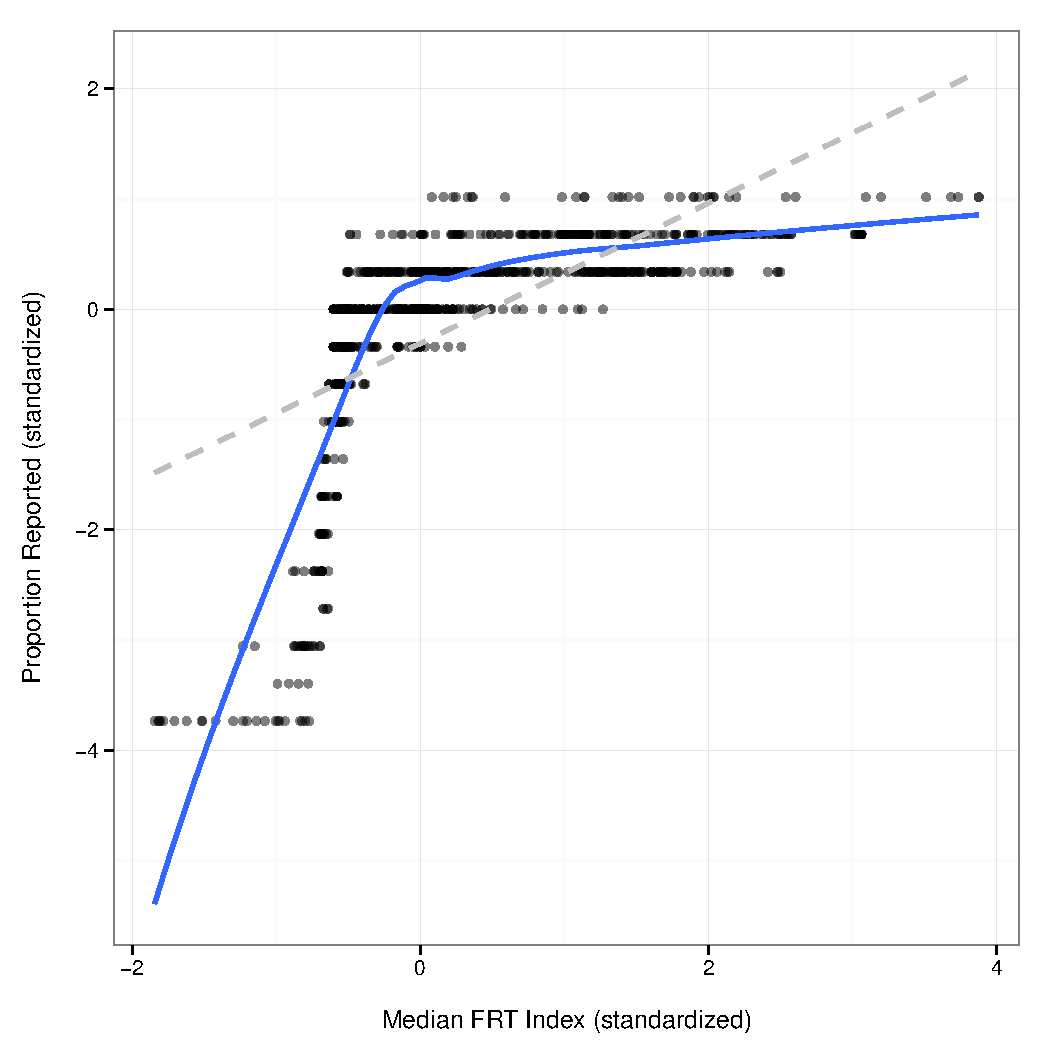
\includegraphics[scale=0.4]{/git_repositories/FRTIndex/paper/paper_plots/FRT_Prop_Compare.pdf}
        \end{center}
    }

    \frame{
        \frametitle{Discrimination parameter}
        How well reporting an item predicts reporting other items.
        \begin{center}
            \includegraphics[scale=0.4]{/git_repositories/FRTIndex/paper/paper_plots/discriminationPlot.pdf}
        \end{center}
    }

    \frame{
        \frametitle{Difficulty parameter}
        On average how well reported is the item.
        \begin{center}
            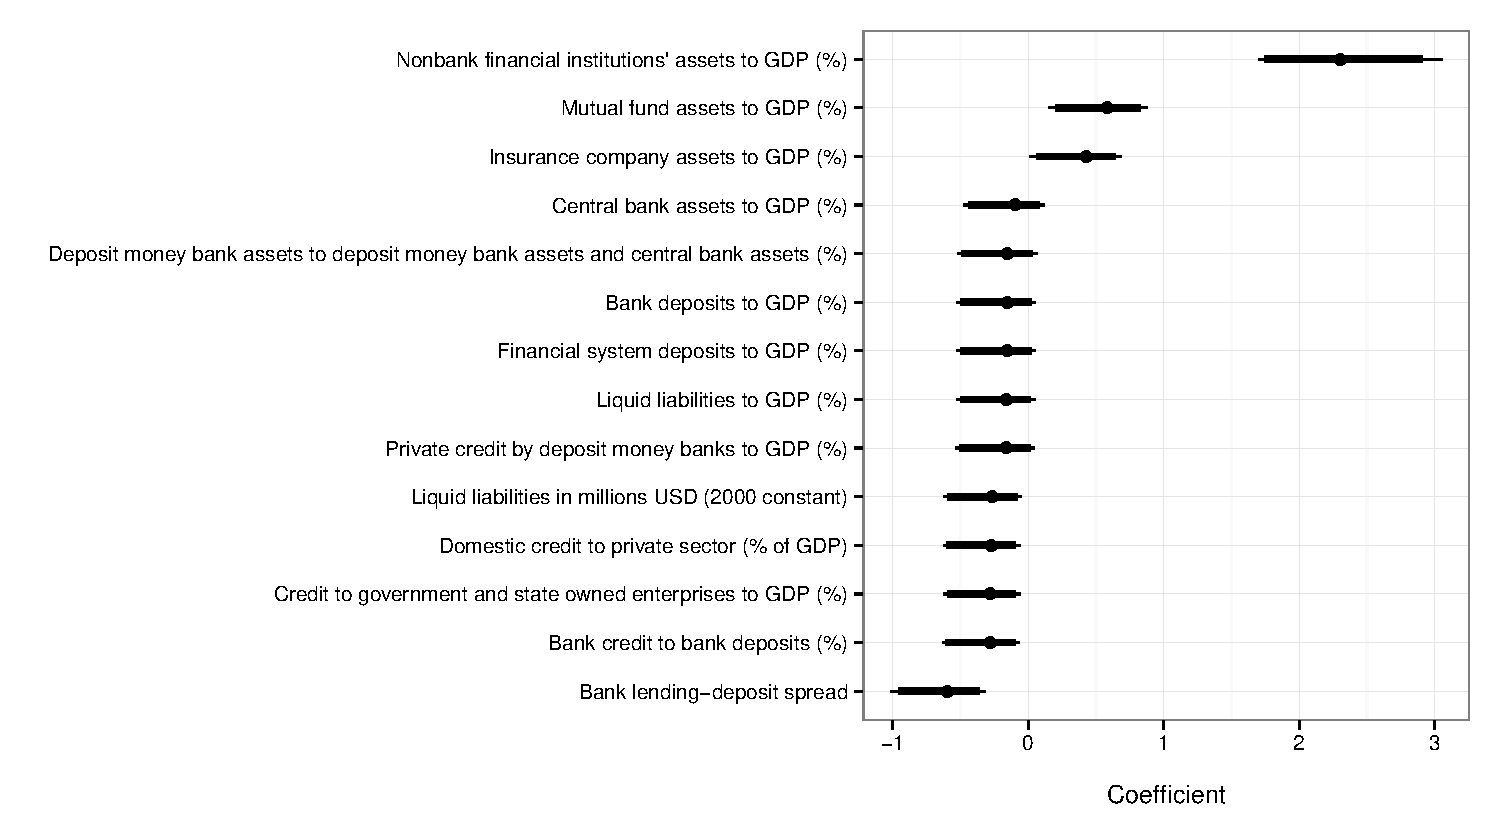
\includegraphics[scale=0.4]{/git_repositories/FRTIndex/paper/paper_plots/difficultyPlot.pdf}
        \end{center}
    }

    \frame{
        \frametitle{Comparison to survey/frequency measures}
        Comparision to Liedorp et al. (2013)
        \begin{center}
            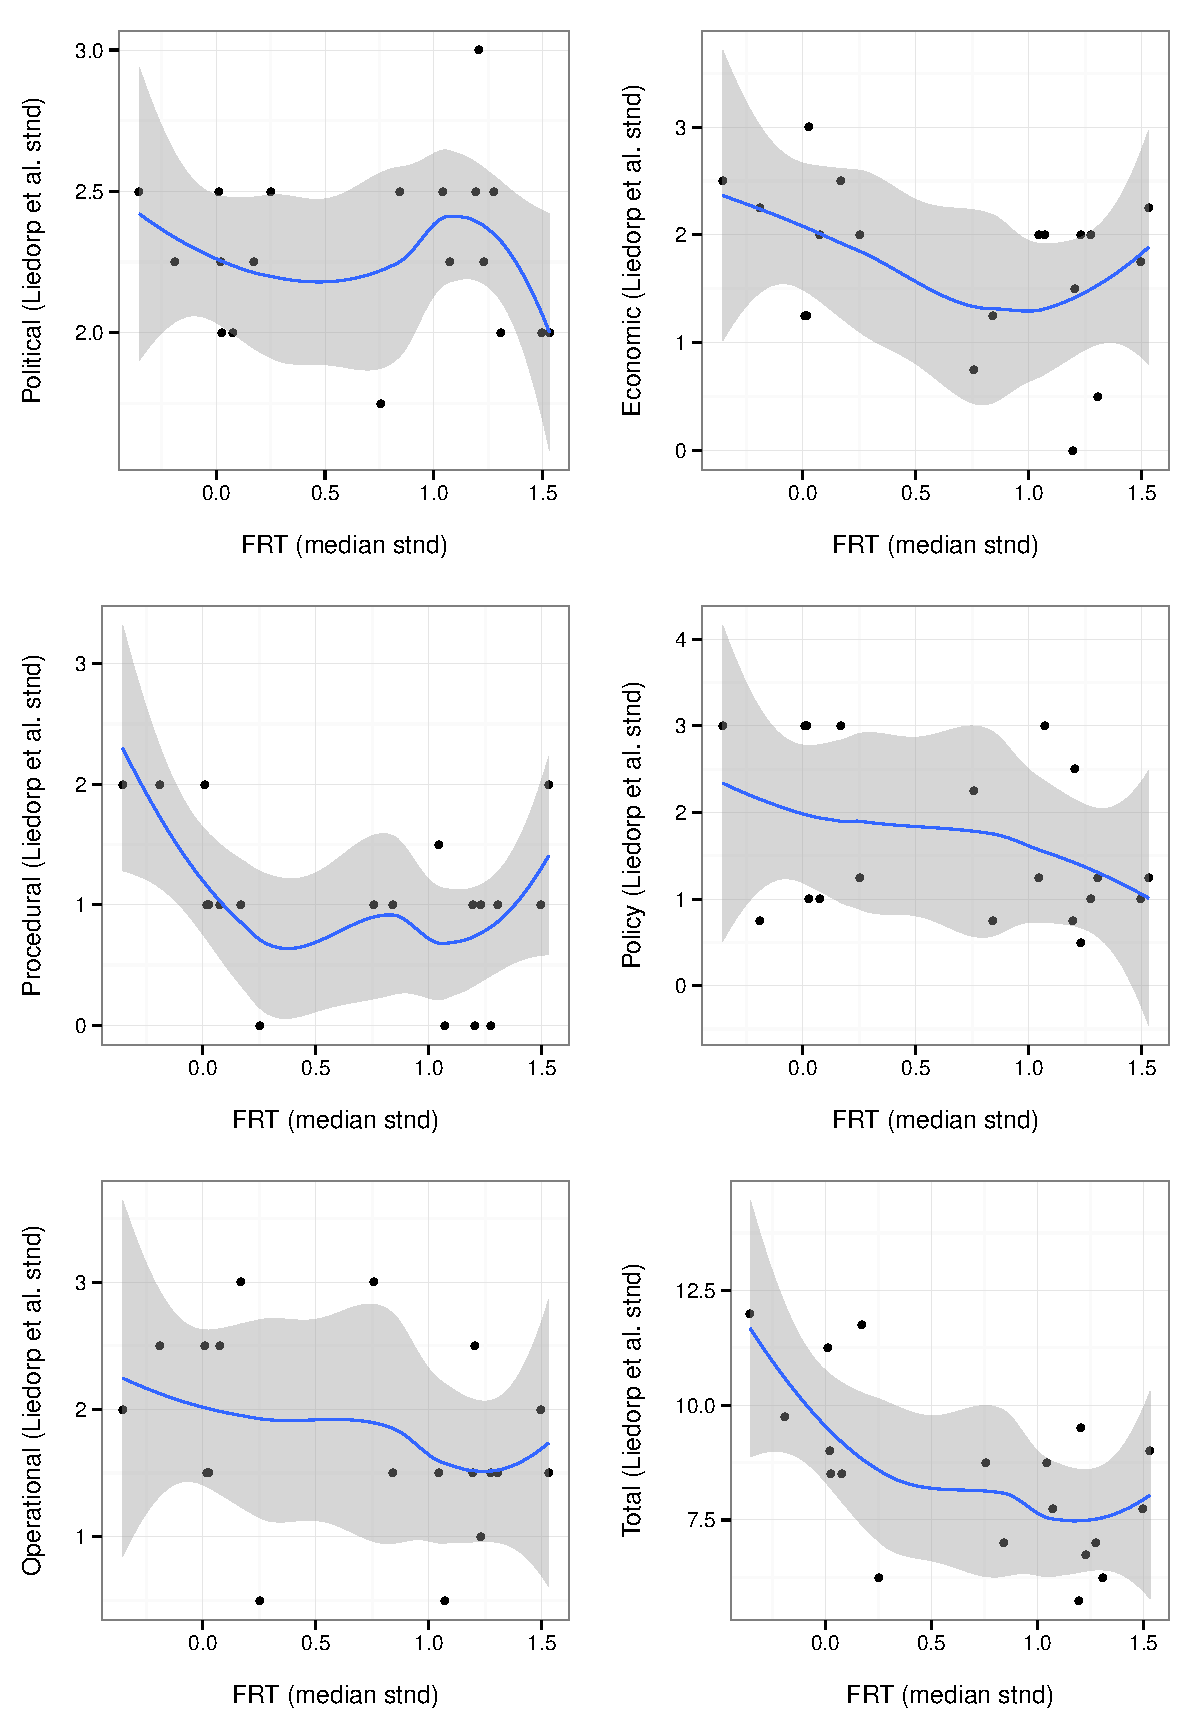
\includegraphics[scale=0.25]{/git_repositories/FRTIndex/paper/paper_plots/FRT_Liedorp.pdf}
        \end{center}
    }
    
    \frame{
    	\frametitle{One annoying issue\ldots}
	There is a possibility that \textbf{missing-ness} is sometimes caused by World Bank \textbf{data handling errors} rather than countries' willingness to report. \\[0.5cm]
	
	For example, Bank Deposits to GDP (\%) is not reported for the UK. However, a \textbf{mirror} of the GFDD (FRED)  \textbf{does have} the data.\\[0.5cm]
	
	\url{http://research.stlouisfed.org/fred2/series/DDOI02GBA156NWDB}
    }

\section{Conclusion}

    \frame{
        \frametitle{To-Do}
        \begin{itemize}
            \item Understand \textbf{why} countries \textbf{increase/decrease} their reporting.
            \item Examine how reporting is associated with economic outcomes:
                \begin{itemize}
                    \item<1-> \textbf{Investment flows}
                    \item<1-> \textbf{Financial stability}
                \end{itemize}
        \end{itemize}
    }


\end{document}
